\documentclass{article}
\usepackage[utf8]{inputenc}
\usepackage{graphicx}

\title{320 Requirements}
\author{Trevor's Team}
\date{\today}

\begin{document}
\begin{titlepage}

\maketitle

\begin{abstract}
\textbf{Purpose of System:} \newline
\newline
The purpose of this system is to be an online tutor for students at the University of Massachusetts Amherst. This learning tool would help teach the students and allow them to create ER diagrams and submit them as homework assignments. They can then be graded by solutions uploaded by the instructor of a course. Feedback will then be provided to help the student learn from their mistakes. The benefits of this system is that it makes submitting learning in the course and submitting homework much easier for both the students and instructor. \newline


\textbf{Scope:}
\newline \newline
This document will clearly outline the requirements and the system requirements of ER Diagram Tutoring System. This document should cover all key concepts and fundamental requirements. The requirements should satisfy the standards of the client and provide accuracy in the functionality of the system. 


\end{abstract}

\end{titlepage}

\tableofcontents
\newpage
\begin{section}{Data Dictionary}
\begin{center}
    \begin{tabular}{ | l | l | l |l| p{5cm} |}
   \hline
    Student Info & Pay Info & New Class & Class Availability \\ \hline

    

    
    - Name          &  - Student ID &  - Student ID           & - Student ID  \\
    - Student ID    &  - Amount     &  - Transcript           & - Class ID  \\ 
    - SSN           &  - Name       &  - Section              & - Seat Availability\\ 
    - Date of Birth &  - Address    &  - Discussion Section   & - Class Capacity   \\ 
    - Address       &  - Phone      &  - Class ID             &   \\ 
    - Telp. Number  &  - EMail      &  - Professor            &   \\ 
    - Gender        &               &                         &   \\ 
    - Email         &               &                         &   \\ 
    - Classes Taken &               &                         &   \\ 
    - Grades        &               &                         &\\ \hline

    
       
    
Proof of Registration & Send Payment Due & Billing Info & Class Roster\\ \hline
       - Student ID   &  - Student ID    &  - Student ID& - Student ID  \\ 
       - Day          &  - Name          &  - Name      & -Name\\
       - Time         &  - Amount        &  - Address   & Major   \\ 
       - Room         &  - Receipt ID    &  - Phone     &   \\ 
       - Class ID     &                  &    - Email   & \\ 
                      &                  &    - Amount  & \\
                      &                  &              &   \\ 
                      &                  &               &\\ \hline
    
    
    
    
    
    
    
    
    
    \hline
    \end{tabular}
\end{center}
\end{section}
\newpage
\iffalse
\begin{section}{Context Level Diagram}
    \begin{figure}[h!]
        \begin{center}
           \centerline{ 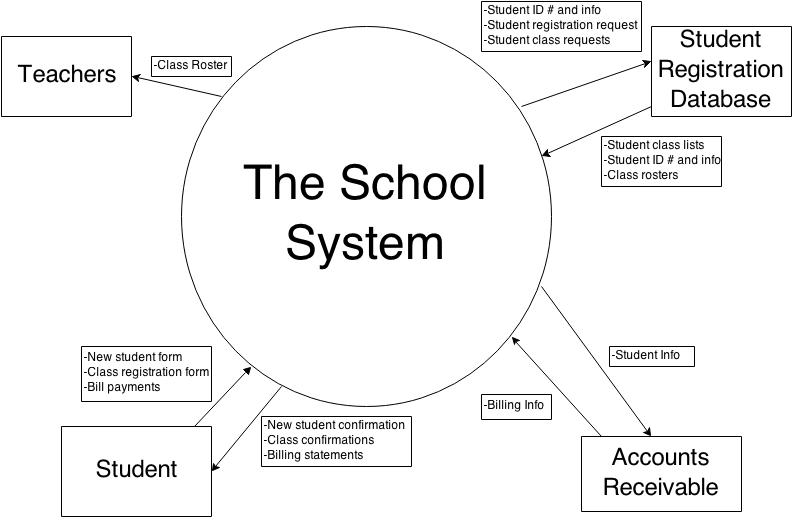
\includegraphics[height=13cm]{DF.jpg}}
            \caption{DFD Context Diagram}
        \end{center}
    \end{figure}
\end{section}
\newpage
\begin{section}{Level 0 Diagram}
    \begin{figure}[h!]
        \begin{center}
            \centerline{\includegraphics[height=13cm]{DFD Level0.jpg}}
            \caption{DFD Level 0 Diagram}
        \end{center}
    \end{figure}
\end{section}
\newpage




















\end{document}
